\chapter{Algorithme 1}

\section{Présentation}

Cet algorithme reprend l'algorithme MCS (ou MCG) classique avec la technique NEE, si ce n'est qu'entre deux points de réflexions on prend en compte l'atténuation de la fumée. Cette prise en compte est également faite entre la source et les différents points de surface, ou entre le récepteur et les différents points de surface.

\section{Intégration continue}

Entre deux points $p$ et $p'$, dans la direction $\omega$ ($p' = p + t\omega$), le rayon passe dans de la fumée et de ce fait nous avons la formule suivante :
\large \begin{equation}
    L_i(p', \omega) = T_r(p \rightarrow p')L_o(p, \omega)
.\end{equation} \normalsize \par
Rappelons ici la défintion de la transmittance $T_r$ (eq. \ref{eq:transmittance_definition}) :
\large \begin{equation}
    T_{r}(p\longrightarrow p') = e^{-\int_{0}^{d} \sigma_{t}(p+t\omega, \omega)dt}
.\end{equation} \normalsize

Dans cet algorithme, c'est le seul calcul que nous ferons, pour chaque luminance sortant d'un point de réflexion (ou de la source) et arrivant sur un autre point de réflexion (ou sur l'émetteur).\par
Rappelons l'équation \ref{eq:Eclairement_LTE_potentiel} pour l'algorithme MCS avec NEE :
\large \begin{multline*}
    E(M_{tx}, M_{rx}, t) =
        \int_{\Omega_{tx}}
            L_e(M_{tx}, \overrightarrow{\omega_0}, t)
            W_l^*(x_1, M_{rx}, t)
            | \overrightarrow{\omega_0} \cdot \overrightarrow{n_{tx}} |
            d\overrightarrow{\omega_0}
        \\ +
        \int_{\Omega_{tx}}
            L_e(M_{tx}, \overrightarrow{\omega_0}, t)
            | \overrightarrow{\omega_0} \cdot \overrightarrow{n_{tx}} |
            \int_{\Omega_1}
                W^*(x_1, M_{rx}, \overrightarrow{\omega_1}, t)
            d\overrightarrow{\omega_0}
        d\overrightarrow{\omega_1}
,\end{multline*} \normalsize
avec
\large \begin{equation*}
    W_l^*(x_1, M_{rx}, t) =
        f_r(x_1, \overrightarrow{\omega_0} \longrightarrow \overrightarrow{x_1 M_{rx}})
        W_l(x_1, M_{rx}, t)
        | \overrightarrow{\omega_1} \cdot \overrightarrow{n_1} |
,\end{equation*} \normalsize
et
\large \begin{equation*}
    W^*(x_1, M_{rx}, \overrightarrow{\omega_1}, t) = 
        f_r(x_1, \overrightarrow{\omega_0} \longrightarrow \overrightarrow{\omega_1})
        W(x_1, M_{rx}, \overrightarrow{\omega_1}, t)
        | \overrightarrow{\omega_1} \cdot \overrightarrow{n_1} |
.\end{equation*} \normalsize \newline \par

En ajoutant la prise en compte de la fumée, nous aurons :
\large \begin{multline}
    E(M_{tx}, M_{rx}, t) =
        \int_{\Omega_{tx}}
            \textcolor{red}{T_r(M_{tx} \rightarrow x_1)}
            L_e(M_{tx}, \overrightarrow{\omega_0}, t)
            W_l^*(x_1, M_{rx}, t)
            | \overrightarrow{\omega_0} \cdot \overrightarrow{n_{tx}} |
            d\overrightarrow{\omega_0}
        \\ +
        \int_{\Omega_{tx}}
            \textcolor{red}{T_r(M_{rx} \rightarrow x_1)}
            L_e(M_{tx}, \overrightarrow{\omega_0}, t)
            | \overrightarrow{\omega_0} \cdot \overrightarrow{n_{tx}} |
            \int_{\Omega_1}
                W^*(x_1, M_{rx}, \overrightarrow{\omega_1}, t)
            d\overrightarrow{\omega_0}
        d\overrightarrow{\omega_1}
,\end{multline} \normalsize
avec
\large \begin{equation*}
    W_l^*(x_1, M_{rx}, t) =
        \textcolor{red}{T_r(x_1 \rightarrow M_{r_x})}
        f_r(x_1, \overrightarrow{\omega_0} \longrightarrow \overrightarrow{x_1 M_{rx}})
        W_l(x_1, M_{rx}, t)
        | \overrightarrow{\omega_1} \cdot \overrightarrow{n_1} |
,\end{equation*} \normalsize
et
\large \begin{equation*}
    W^*(x_1, M_{rx}, \overrightarrow{\omega_1}, t) = 
        f_r(x_1, \overrightarrow{\omega_0} \longrightarrow \overrightarrow{\omega_1})
        W(x_1, M_{rx}, \overrightarrow{\omega_1}, t)
        | \overrightarrow{\omega_1} \cdot \overrightarrow{n_1} |
,\end{equation*} \normalsize
où
\large \begin{equation*}
    W(x, y, \overrightarrow{\omega_x}, t) =
        \textcolor{red}{T_r(x \rightarrow y)}
        W_e(x, y, \overrightarrow{\omega_x}, t) +
        \int_{\Omega_z}
            f_r(z, \overrightarrow{\omega_x} \longrightarrow \overrightarrow{\omega_z})
            W(z, y, \overrightarrow{\omega_z}, t)
            |\overrightarrow{\omega_z}, \overrightarrow{n_z} |
        d\overrightarrow{\omega_z}
.\end{equation*} \normalsize

\section{Implémentation discrète}

Cette intégrale peut être transformée avec Monte Carlo :

\large \begin{multline}
    E_k(M_{tx}, M_{rx}, t) =
    \frac{1}{N}
    \underbrace{
        \sum\limits_{s=1}^N \frac
            {| \overrightarrow{\omega_0} \cdot \overrightarrow{n_{tx}} |
             \textcolor{red}{T_r(M_{tx} \rightarrow x_1)}
             L_e(M_{tx}, \overrightarrow{\omega_{tx}}, t)}
            {p_0(M_{tx}, \overrightarrow{\omega_0})}
        }
        _{\textcolor{DarkGray}
         {\substack{\text{On tire une première} \\
                    \text{direction pour $\overrightarrow{\omega_0}$}}}}
    \\ \times
    \sum \limits_{i=1}^k
    \left(
        \underbrace
            {W_l(x_i, M_{rx}, t)}
            _{\textcolor{DarkGray}
             {\substack{\text{Contribution} \\
                        \text{directe du} \\
                        \text{point $x_i$ sur} \\
                        \text{le récepteur}}}}
        \underbrace
            {\prod\limits_{j=1}^i
                \frac{
                    \textcolor{red}{T_r(x_j \rightarrow x_{j-1})}
                    f_r(x_j, \overrightarrow{\omega_{j-1}} \longrightarrow \overrightarrow{\omega_{j}})
                    | \overrightarrow{\omega_j} \cdot \overrightarrow{n_j} |}
                    {p_j(x_j, \overrightarrow{\omega_{j}})}}
                _{\textcolor{DarkGray}
                 {\substack{\text{Prise en compte de toutes les BRDF} \\
                            \text{des surfaces interceptées, et de la} \\
                            \text{fumée entre les différents sommets du chemin}}}}
    \right)
.\end{multline} \normalsize



\section{Algorithme}

Dans ma classe \textbf{ParticipatingMedia}, j'ai ajouté la méthode \textbf{\textit{multiplyByTransmittance}} qui, pour une distance $d$ donnée, multiplie des champs par la transmittance $tr = e^{-\sigma_t d}$ (possible car nous sommes dans un milieu homogène).\par
Ensuite, cette méthode est appliquée sur chaque rayon produit par l'algorithme de lancer de rayons.

\section{Résultats}

Dans cet algorithme, puisque le seul impact de la fumée est l'extinction par la transmittance, nous n'avons pas à différencier les coefficients d'atténuation $\sigma_a$ et de dispersion $\sigma_s$. En effet, le seul qui nous intéresse est $\sigma_t = \sigma_a + \sigma_s$.\par
Les résultats qui suivent ont été réalisés avec $10^8$ rayons lancés, 3 réflexions, et 4 valeurs différentes de $\sigma_t$. Ils sont présentés dans un premier temps, par réflexion (seulement le trajet direct, seulement la première réflexion, ...) puis toutes les contributions sont rassemblées.

\begin{center}
\begin{figure}[h!]
      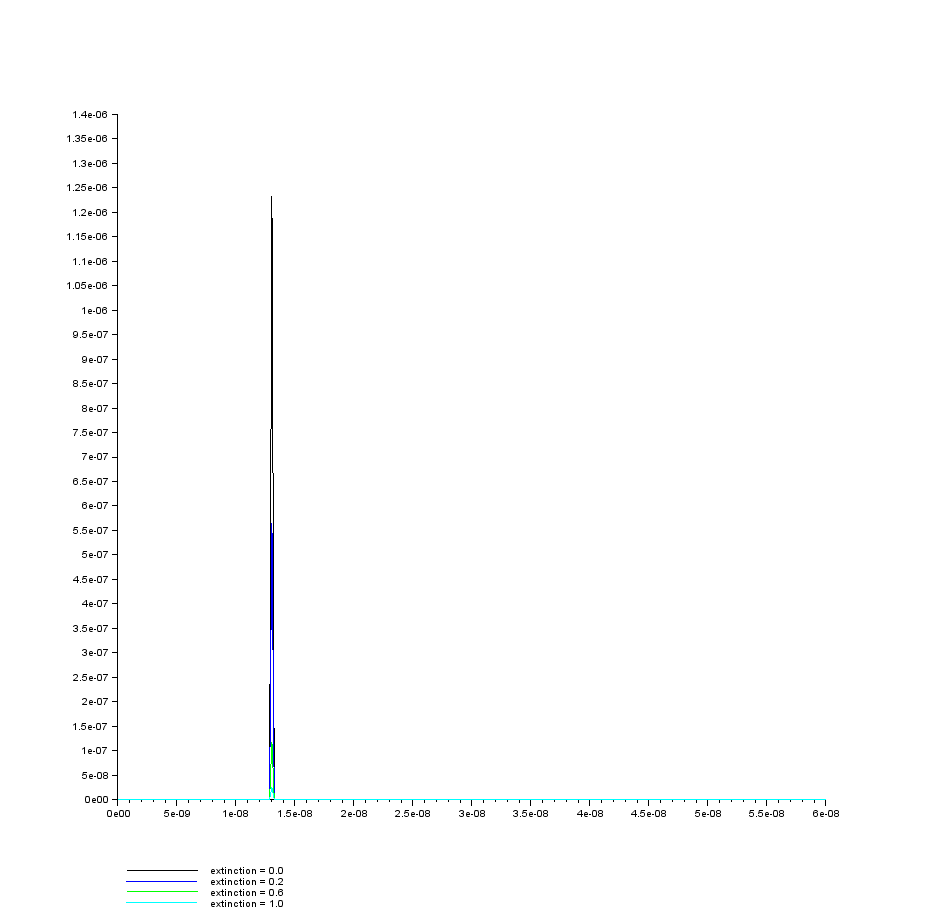
\includegraphics[width = 180mm]{resultats/algo1/depth0.png}
      \caption{k = 0}
\end{figure}
\begin{figure}[h!]
      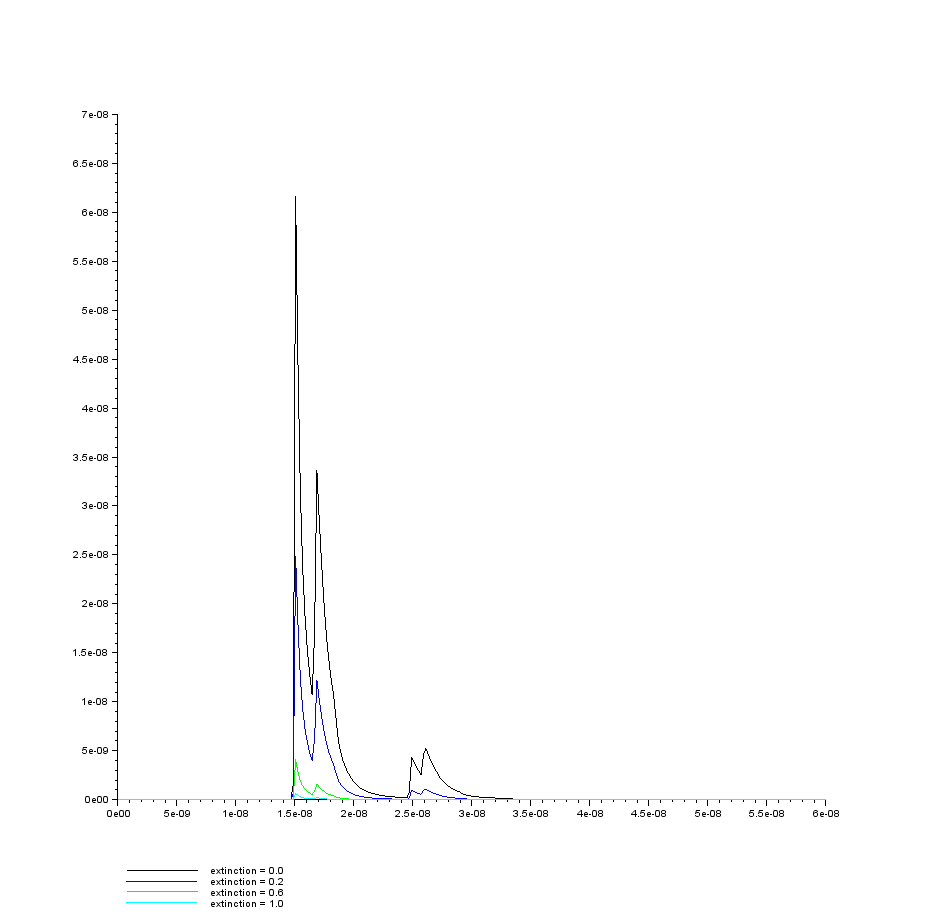
\includegraphics[width = 19cm]{resultats/algo1/depth1.png}
      \caption{k = 1}
\end{figure}
\begin{figure}[h!]
      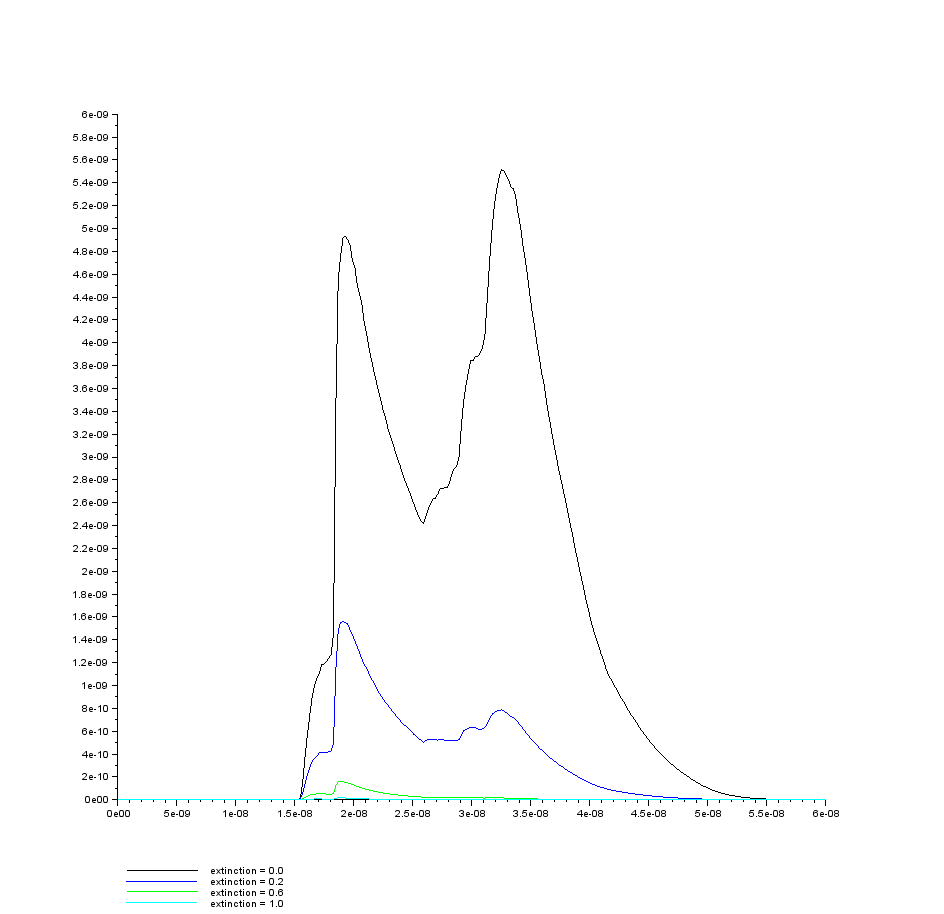
\includegraphics[width = 19cm]{resultats/algo1/depth2.png}
      \caption{k = 2}
\end{figure}
\begin{figure}[h!]
      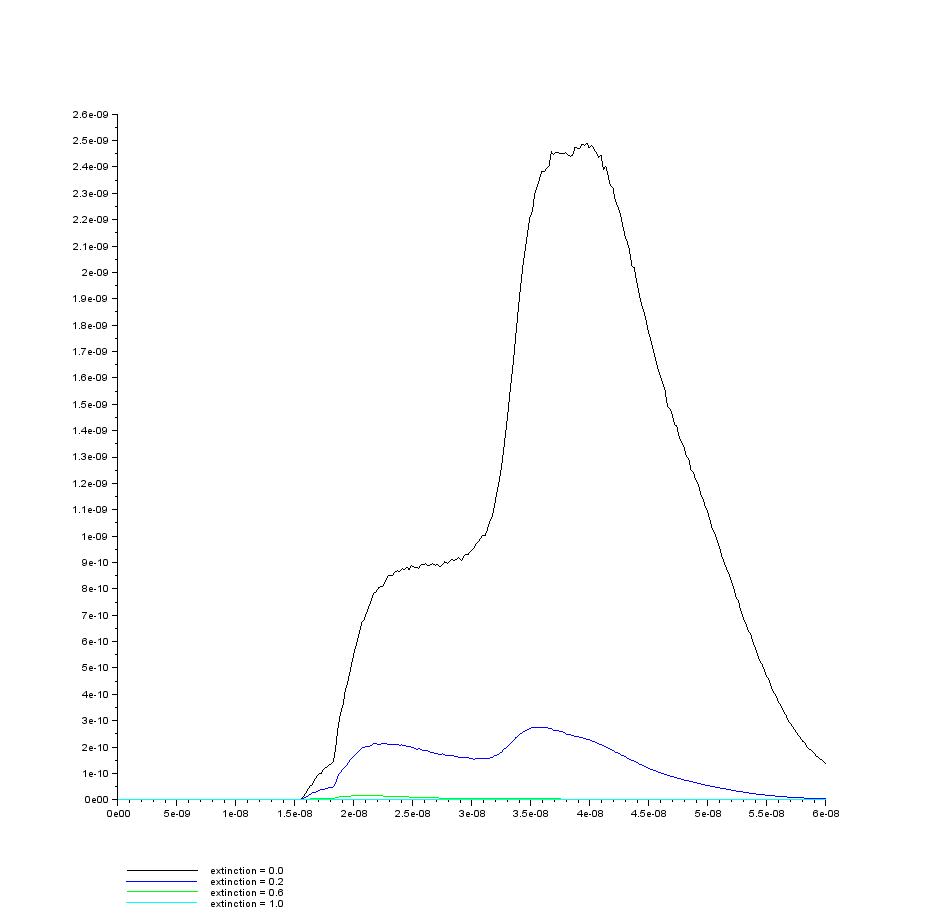
\includegraphics[width = 19cm]{resultats/algo1/depth3.png}
      \caption{k = 3}
\end{figure}
\begin{figure}[h!]
      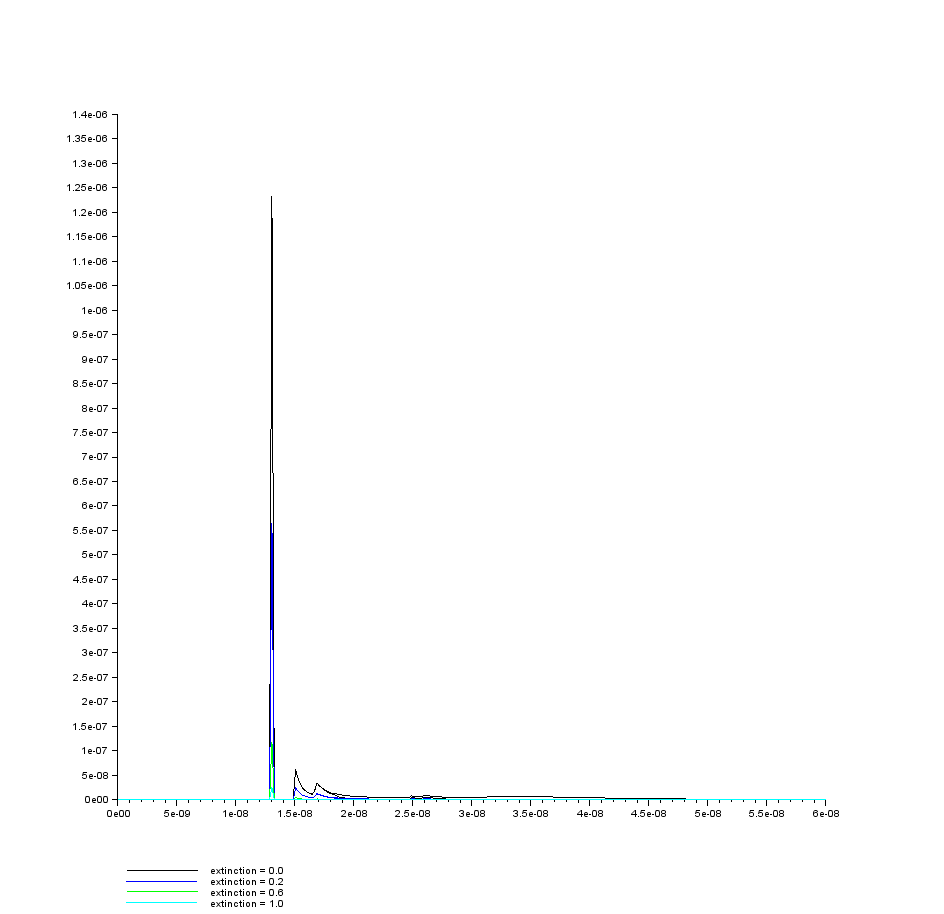
\includegraphics[width = 19cm]{resultats/algo1/alldepth.png}
      \caption{k = 0, 1, 2, 3}
\end{figure}
\end{center}